\documentclass[a4paper]{article}
\usepackage[T1]{fontenc}
\usepackage[utf8]{inputenc}
\usepackage{lmodern}
\usepackage{graphicx}

\usepackage[english]{babel}

\title{Survey Project :\\Report}
\author{Marguerite Rince}

\begin{document}
\maketitle
\paragraph{}
During last few weeks, we have been conducting a survey about download the phenomena of download. Indeed nowadays, our society is passing through an internet crisis. One of the most significant  examples, is the recent closure of the most famous download platform : MegaUpload. This controversial measure taken by the American government shows, how wide spread downloading is in our society. 

In this context, we wanted to learn how people see the download's evolution and how much important it is for them. However, conducting a traditional survey (asking people questions in the street) was not the solution here. In fact, people could have been frightened of telling the truth about awkward questions. So we have thought that an online questionnaire might been a good way to have a large number of fair answers.

The main goal of this survey is to know if the big cliche of the common downloader is actually right : a rebel teenage who download music and video games. If not, who are those downloaders, why do they download, and what are their opinions of the vain attempts of download law ?


\clearpage
\paragraph{}
From the outset, the first graph answer no to the big question. Indeed, we learn that people between  30 and 45 years old are the ones who download most often. Of course, they are closely followed by the youngest. People older than 50 years, as we could presumed, come in last postion and a third of them never dowload.
\begin{figure}[htbp]
  \centering
  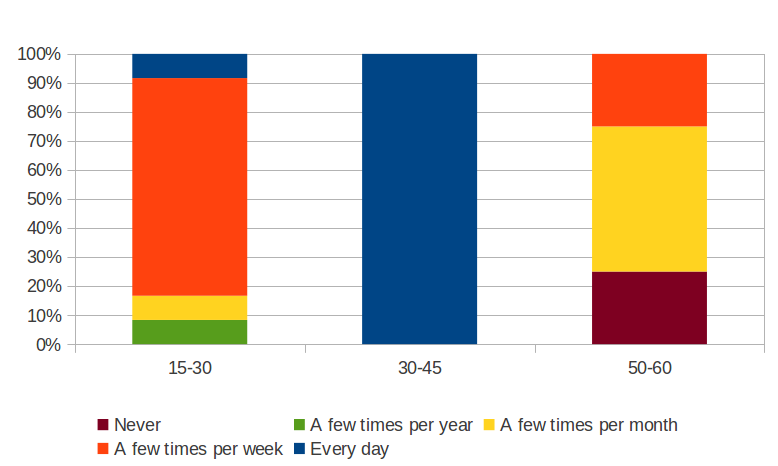
\includegraphics[scale=0.40]{graph1}
  \caption{Graph1}
  \label{fig:Graph1}
\end{figure}  

\paragraph{}
Our second graph is a bar chart which illustrates how men and women download. The results show that there are no differences between men and women. Indeed both of them download (only 10\% say that they don't) legally and illegally. Nevertheless, our hypothesis about the type of download is confirmed. Almost 80\% of people download illegally. Even if people use the legal way, it is only 20\% of those are questioned.
\begin{figure}[htbp]
  \centering
  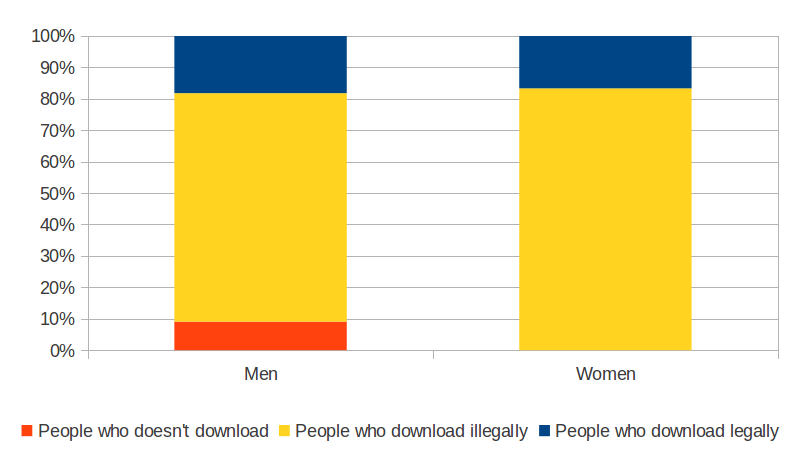
\includegraphics[scale=0.30]{graph2}
  \caption{Graph2}
  \label{fig:Graph2}
\end{figure}
\paragraph{}
According our third graph, movies are the main target of downloaders (90\% of them), closely followed by music with with 78\%. These results show that there are only two common categories among downloaders since movies and music are products used by every age. Contrary to games, software or ebooks that are more specific and allow us to define a profile. 
\begin{figure}[htbp]
  \centering
  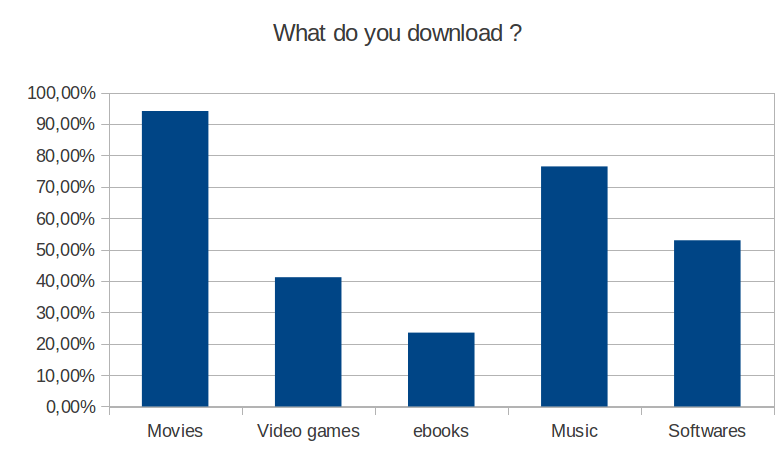
\includegraphics[scale=0.40]{graph3}
  \caption{Graph3}
  \label{fig:Graph3}
\end{figure}
\paragraph{}
This ways, the fourth graph confirm that downloaders have the same demands that normal customers have  : price and access to the product. These two key points which made the success of the supermarket, are responsible of the dowload's sucess too.
\begin{figure}[htbp]
  \centering
  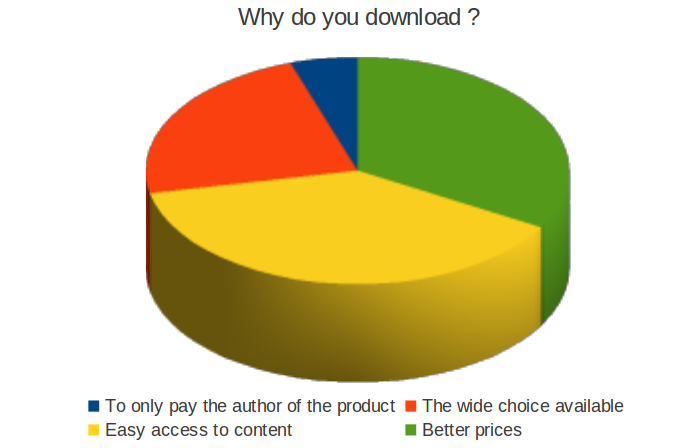
\includegraphics[scale=0.40]{graph4}
  \caption{Graph4}
  \label{fig:Graph4}
\end{figure}
\paragraph{}
The next graph is a bart chart which clearly identifies people's opinion about actual download laws. About 55\% of them think that they are useless. Moreover, the second score (29\%) is the percentage of people who are not aware of it. 







\begin{figure}[htbp]
  \centering
  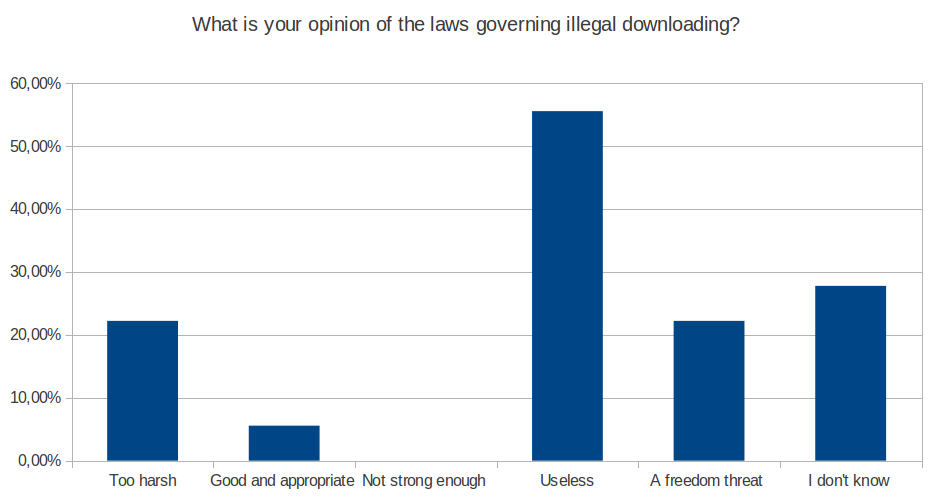
\includegraphics[scale=0.40]{graph5}
  \caption{Graph5}
  \label{fig:Graph5}
\end{figure}
\begin{figure}[htbp]
  \centering
  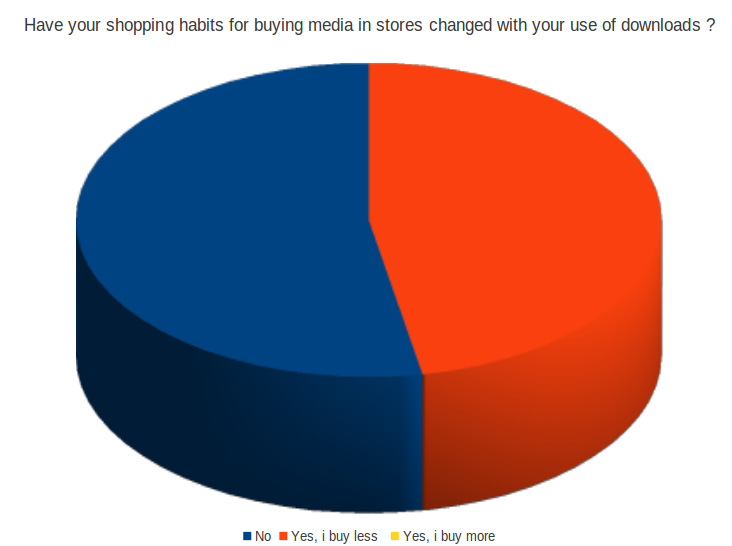
\includegraphics[scale=0.40]{graph6}
  \caption{Graph6}
  \label{fig:Graph6}
\end{figure}
\end{document}


